\author{Gilles Hennenfent\/\footnotemark[1] and Sergey Fomel\/\footnotemark[2]}
\title{Madagascar for reproducible scientific publications tutorial}

\lefthead{Hennenfent \& Fomel}
\righthead{Reproducible scientific publications}

\newcommand{\rsf}{\textsf{Madagascar}\ }

\footnotetext[1]{Department of Earth \& Ocean Sciences, University of British Columbia at Vancouver. Email: ghennenfent@eos.ubc.ca}
\footnotetext[2]{Bureau of Economic Geology, University of Texas at Austin. Email: sergey.fomel@beg.utexas.edu}


\maketitle

\begin{abstract}
   xxx
\end{abstract}

\section{Introduction}

\rsf (formerly known as \textsf{RSF}) is an open-source software
package for reproducible geophysical data processing and computational
experiments. Its mission is to provide a simple yet powerful
environment and technology transfer tool for researchers working with
digital image and data processing. The technology developed using the
\rsf package is transferred in the form of recorded processing flows,
which become documented "computational recipes" to be verified,
exchanged, and modified by the entire \rsf community.

\subsection{Structure of a reproducible scientific publication}

\begin{figure}[h]
\begin{center}
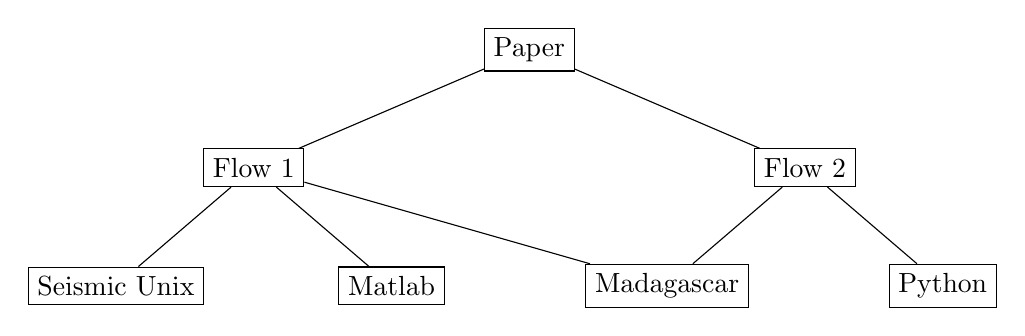
\begin{tikzpicture}
\tikzstyle{every node}=[rotate=0,draw]
\tikzstyle{level 1}=[sibling distance=70mm]
\tikzstyle{level 2}=[sibling distance=35mm]
\node (paper) {Paper}
child {node (flow 1) {Flow 1}
  child{node (su) {Seismic Unix}}
  child{node (matlab) {Matlab}}
}
child {node (flow 2) {Flow 2}
  child{node (rsf) {Madagascar}}
  child{node (python) {Python}}
};
\draw (flow 1) -- (rsf); 
\end{tikzpicture}

\end{center}
\caption{Structure of a \rsf reproducible document}\label{fig:struct}
\end{figure}

\subsection{How to read this tutorial}
\subsection{Authors and Acknowledgments}
\subsection{Getting help}

\section{Writing a reproducible scientific publications}
\subsection{SCons for processing flows}

Example of how to integrate Matlab, (Mathematica,) and Python would be
nice.

\subsection{\LaTeX\ document}
\subsubsection{SConstruct file}
Show how to Fetch non-repro figures.

\subsection{Website}

Construct a website from the \LaTeX\ document.

%%% Local Variables: 
%%% mode: latex
%%% TeX-master: t
%%% End: 
